\documentclass[handout]{beamer}

\usepackage{graphicx, subfigure}
\usepackage{amsmath}


% \usepackage{beamerthemesplit} // Activate for custom appearance

\title{\color{blue} The Street Score project: Scope for Improvement? }
\subtitle{\color{magenta}Knowledge Lab Team Presentation}
\author{ Nandana Sengupta}
\date{\color{blue}\today}


\begin{document}


\frame{\titlepage}
\frame{\titlepage}

\frame{
\frametitle{The Street Score Project}
\begin{itemize} \small

\item<2-> MIT Media Lab Project
\item<3-> Generating database of visual perceptions of safety/uniqueness etc
\item<4-> 
\includegraphics[width = 0.75\textwidth]{streetscore}
\item<5-> Participants shown \textbf{random} pairs of images
\item<6-> {\color{magenta}Main application:} ranking of neighborhoods/ cities.
\item<8-> {\color{magenta}Cities in dataset:} Boston, NYC, Linz, Salzburg
\item<9-> Number of images: 4109 , Number of participants: 7872 , Number of comparisons: 208738. 

\end{itemize}


}






\frame{
\frametitle{Limitations }

\begin{itemize} \small
\item<2->  Google Street View -- represents the way cities look from a car

\item<3->  Early mornings -- less traffic, people, shops closed

\item<4-> Not taking advantage of similarity in images or participants

\item<5->  Sparsity of win-loss matrix, multiple images at the same location

\item<6-> Prediction accuracy 

\item<5-> {\color{magenta}We focused on a single city Boston}
\begin{itemize}

\item<6-> 1237 images from 635 unique locations

\item<7->  Less sparse than overall matrix but still not enough observations for consistent ranking

\item<3->  Multiple images at the exact location
\end{itemize}

\end{itemize}


}






\frame{
\frametitle{Feature Extraction}
\begin{itemize} \small


\item<1-> {\color{magenta}Visual Feature Extraction }

\begin{itemize} \small
\item<2-> MIT's Places CNN (Convolution Neural Networks)

\item<3-> Deep Learning Software, open source

\item<4-> Scene Recognition: 205 scene categories eg, residential, highway, apartments etc.

\item<5-> User Input: Raw Image
\end{itemize}

\item<1-> {\color{magenta}Demographic Feature Extraction }

\begin{itemize} \small
\item<6-> US Census Data and American Community Survey Database 

\item<7-> Demographic characteristics by region, eg, average income, educational levels, racial distribution etc 

\item<8-> User Input: Latitude and Longitude
\end{itemize}

\end{itemize}


}




\frame{
\frametitle{Feature Extraction using Deep Learning Software}

\begin{center}

\textbf{Top 3 Predictors:} (office building, apartment building, hospital ) \\


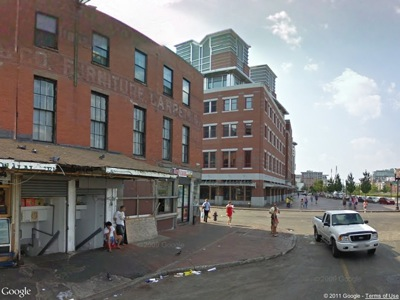
\includegraphics[width = 0.4\textwidth]{id_1_400_300.jpg}

\textbf{Top 3 Predictors:}(yard, residential neighborhood,  driveway) \\

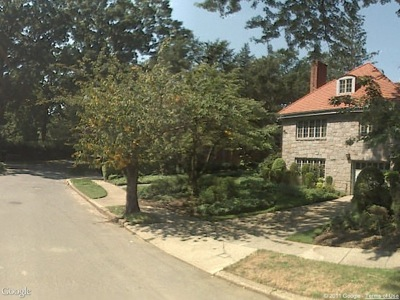
\includegraphics[width = 0.4\textwidth]{id_272_400_300.jpg}



\end{center}



}



\frame{
\frametitle{Feature Extraction: distribution across physical area}


\begin{center}
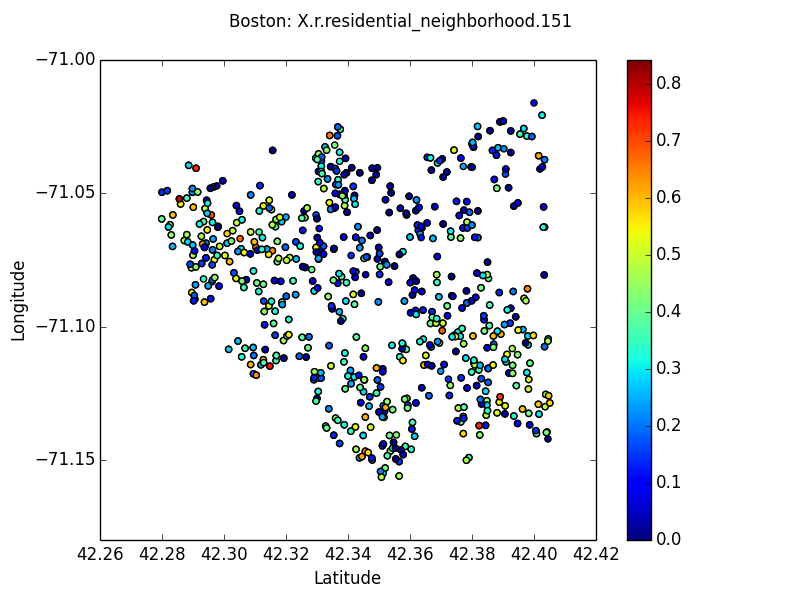
\includegraphics[width = 0.85\textwidth]{bosres}


\end{center}
}


\frame{
\frametitle{Feature Extraction: distribution across physical area}


\begin{center}

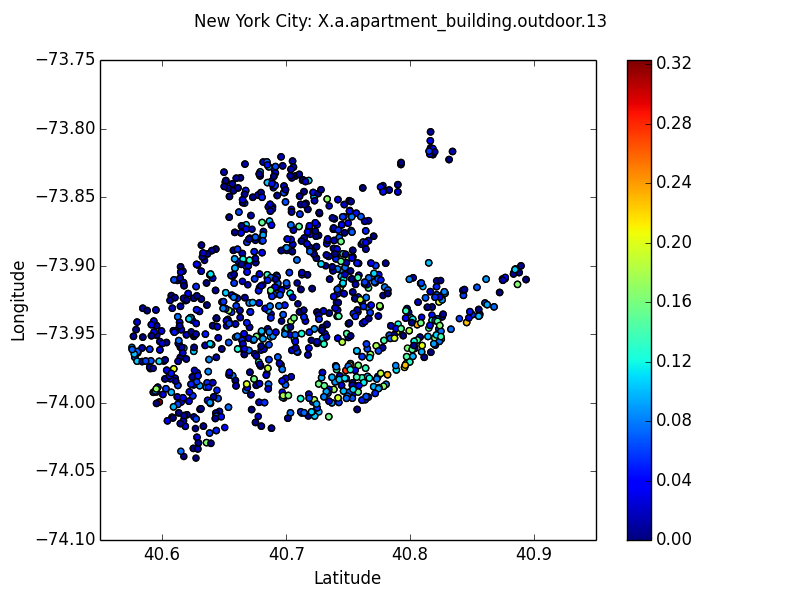
\includegraphics[width = 0.85\textwidth]{nycapart}

\end{center}




}






\frame{
\frametitle{Clustering?}


\begin{itemize}
\item<8->  Divided Boston images into 100 clusters (k-means clustering) 

\item<9-> Features for each cluster: weighted average of member images

\end{itemize}


\begin{center}

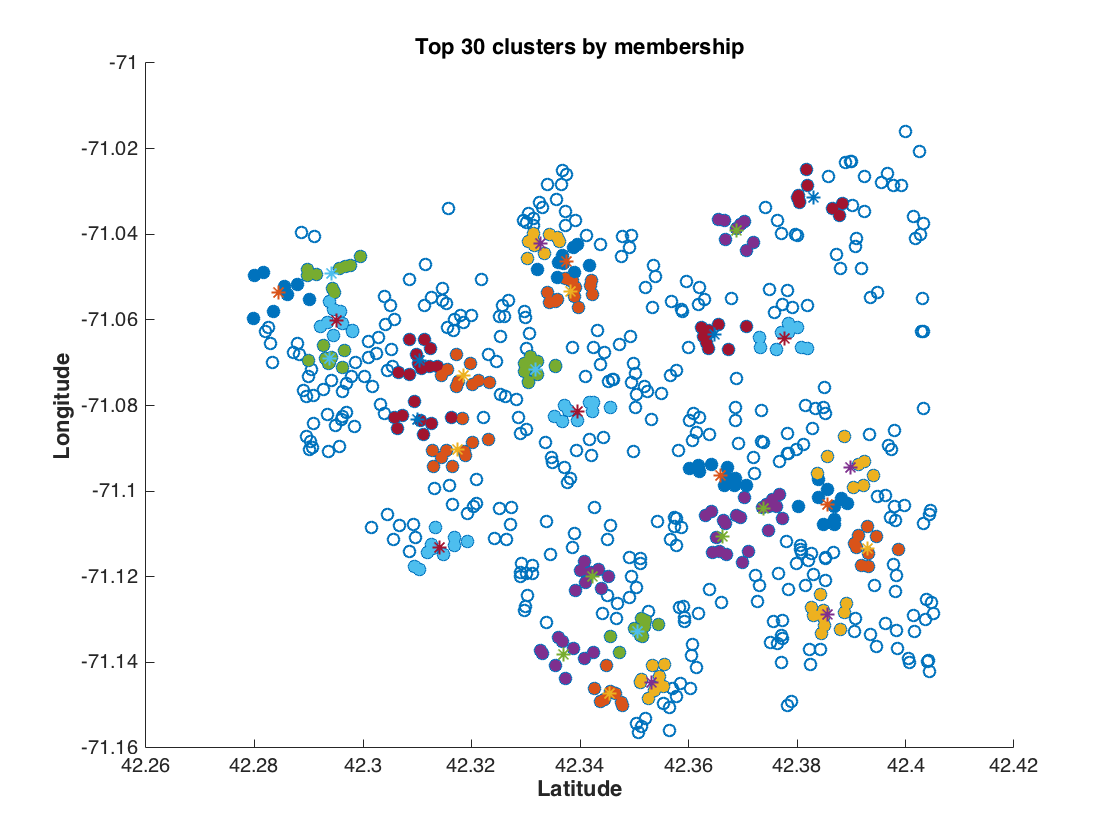
\includegraphics[width = 0.75 \textwidth]{boston_clusters}

\end{center}






}















\end{document}
